% Kapitel 1
% Die Unterkapitel können auch in separaten Dateien stehen,
% die dann mit dem \include-Befehl eingebunden werden.
%-------------------------------------------------------------------------------

\chapter{Einleitung}
%Hier Einleitungstext einfügen, dabei die Formatierungen selber erstellen
Hier ist die Arbeitsweise des Systems anhand von State-Charts darzustellen und
kurz zu erläutern.
\section{Projektdetails}
Die Details der Aufgabenstellung bitte anhand von Statecharts darstellen und
kurz verbal beschreiben.

\subsection{GUI}
Über das GUI soll der Anwender in der Lage sein, dass Programm mit allen vorhandenen Funktionen zu bedienen.
Nach dem Programmstart befindet sich der Anwender in einem Initialzustand. Hierbei sind die Felder des 2D-Modells und der 3D-Darstellung noch leer und die Physikparameter haben Ihre Initialwerte. Man ist in der Lage die Konstruktionsdaten aus dem Editor zu laden um die Bahn erstellen zu können.
Ist dies geschehen, befindet sich der Anwender in der Vorschau. Hier wird ein 2D-Modell der Bahn angezeigt und es können noch Änderungen an den Grafikeinstellungen, sowie den Physikparametern vorgenommen werden. Das Feld der 3D-Darstellung ist weiterhin leer. Aus der Vorschau heraus kann nun auch die Simulation gestartet werden.
Wurde die Simulation gestartet, erscheint sie in dem dafür vorgesehenem Feld. Bei Bedarf kann sie auf Bildschirmgröße maximiert werden. Während der laufenden Simulation können die Simulationsparameter angepasst werden.
Wird die Simulation gestoppt, befindet man sich wieder in der Vorschau, von wo aus man mit dem Schließen der Konstruktion wieder in den Initialzustand gelangt.

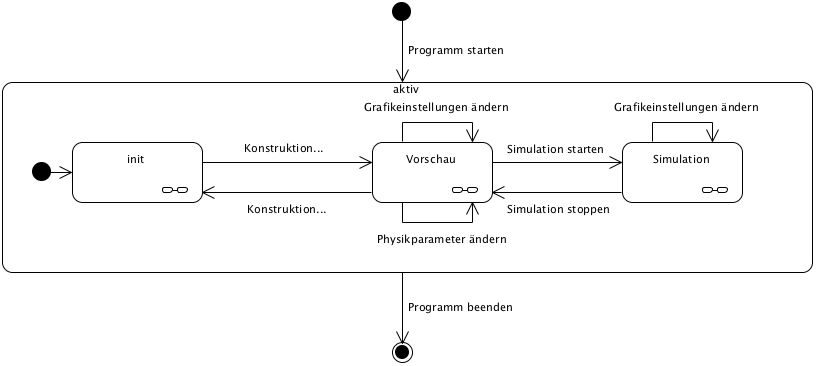
\includegraphics[width=\linewidth]{bilder/StateChart_GUI}

\subsection{Simulator}
Der Simulator dient zur Simulation der Achterbahnfahrt. Er bekommt die Bahndaten von der PhysicsEngine und reicht diese zur Darstellung an die 3D-GraphicsEngine weiter.
\subsection{3D-GraphicsEngine}
Die 3D-GraphicsEngine dient der Visualisierung der Achterbahnfahrt. Sie zeigt die Bahn als 3DModell an und aktualisiert die Kameraposition gemäß der Daten der PhysicsEngine. 


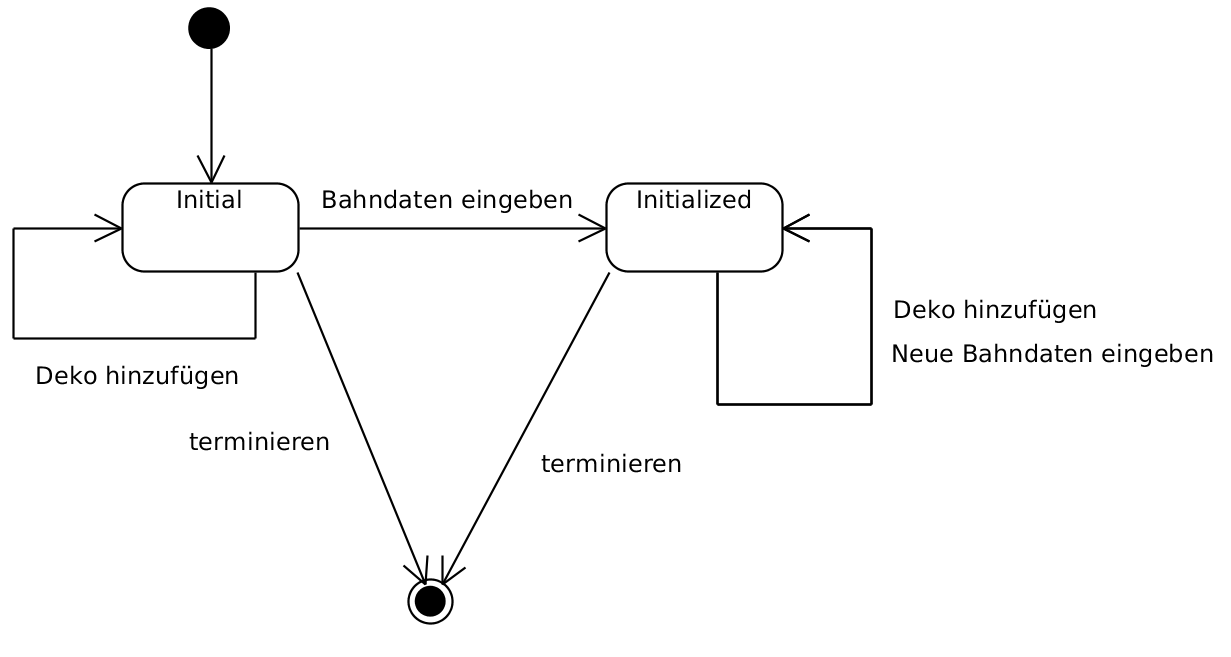
\includegraphics[width=\linewidth]{bilder/statechart_3dgraphics}

Im Initialzustand ist es in Ermangelung von Daten nicht möglich eine Szene zu rendern. Durch eingabe der Bahndaten wird diese Möglichkeit erreicht, jedoch ist zusätzlich ein Startbefehl notwendig,
bevor tatsächlich Regelmäßig Bilder erzeugt werden. Im Savestate ist es dazu von allen Zuständen ohne Zustandswechsel möglich Deko hinzuzufügen, die Grafischen Einstellungen zu ändern oder die Komponente zu terminieren.
In der kritischen Phase des Renderings kann die Komponente nicht unterbrochen werden und auch die veränderung von Einstellungen oder der Deko ist unzulässig. Diese Restriktion dient der verhinderung undefinierter
Zustände bei der Darstellung (im Bilderzeugungsprozess wird die Szene verändert)  und der sauberen Kommunikation mit dem 3D-Hardwarekontext.

\subsection{Mathematics}
Die Mathematik-Komponente stellt Hilfsmethoden zur Berechnung der physikalischen Größen zur Verfügung. Sie wird bei Bedarf durch die Physics Engine aufgerufen und hat daher keinen Lebenszyklus. Eine Visualisierung durch ein Statechart-Diagramm ist somit nicht angebracht.